\chapter{Incorrectly Classified Single Puzzle Images}\label{chap:incorreclyClassifiedSingleImages}

The Mixed-Bag Solver's ability to determine the number of ground-truth images passed to the solver was tested using the Pomeranz \textit{et al.} dataset~\cite{pomeranzBenchmarkImages} containing 20 images each with 805 pieces.  This test measures the performance ceiling of the solver to determine the number of input puzzles.  

The Mixed-Bag Solver (MBS) correctly identified that was only a single ground-truth input for 17 out of the 20 images.  Figure~\ref{fig:groundTruthSingleImageIncorrectlyIdentified} shows the three images that the Mixed-Bag Solver were unable to identify being a single image.  Figure~\ref{fig:mixedBagSolverOuputsSingleImageIncorrectlyIdentified} contains the Mixed-Bag Solver's output for these images; clearly, the solver struggled with the large areas of the image where there was little variation (e.g., blue sky, smooth water).  Paikin~\& Tal note in~\cite{paikin2015} that their assembler does not perform well on such images.  Therefore, it is expected the Mixed-Bag Solver's performance on these images may have improved had a different assembler been used.

\begin{figure}
\centering
  \begin{tabular}{ >{\centering\arraybackslash}m{0.47\textwidth}}

	\fbox{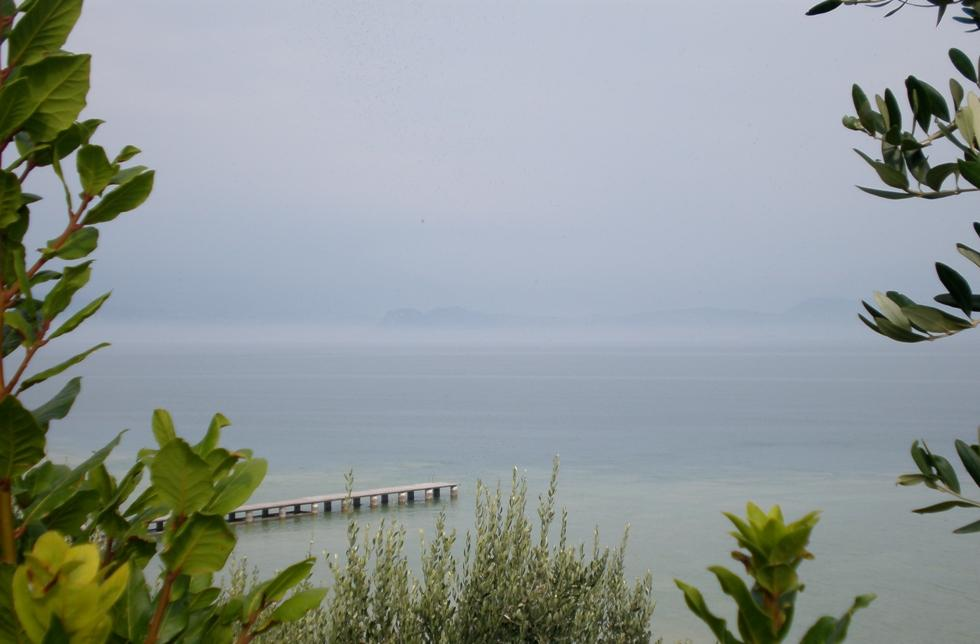
\includegraphics[scale=0.18]{./images/single_puzzle/pomeranz_805_3.jpg}} \\~\\
	Input Image~(a) \\~\\
	\fbox{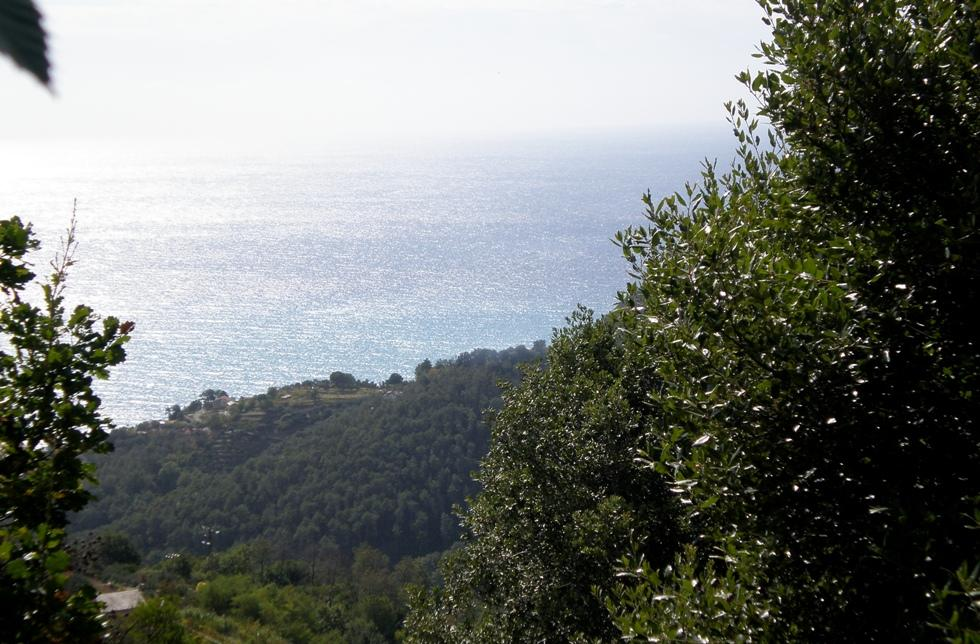
\includegraphics[scale=0.18]{./images/single_puzzle/pomeranz_805_12.jpg}} \\~\\
	Input Image~(b) \\~\\
	\fbox{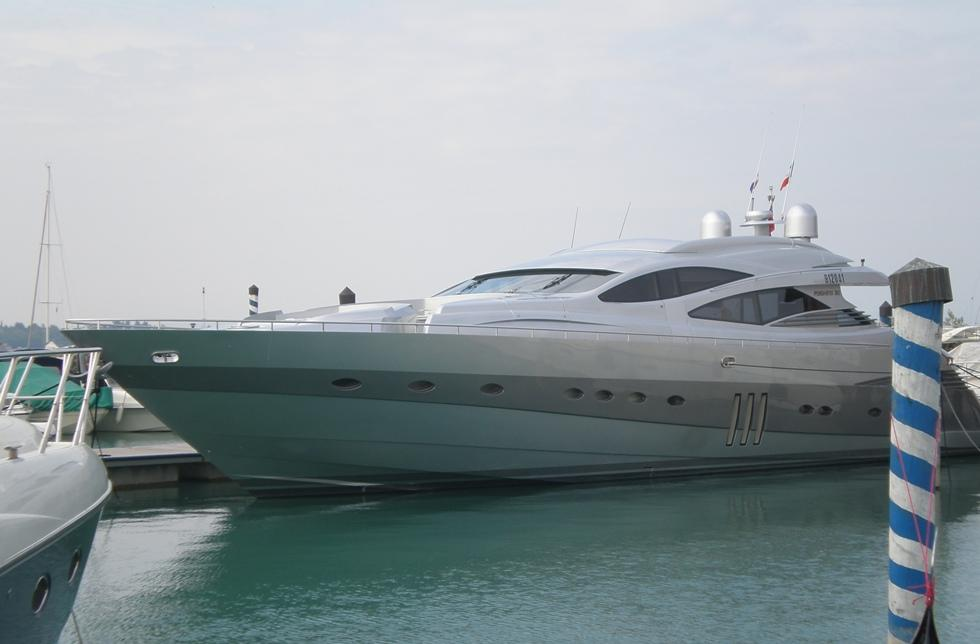
\includegraphics[scale=0.18]{./images/single_puzzle/pomeranz_805_16.jpg}} \\~\\
	Input Image~(c) \\~\\
  \end{tabular}

\caption{805 Piece Images that were Incorrectly Identified by the Mixed Bag Solver}
\label{fig:groundTruthSingleImageIncorrectlyIdentified}
\end{figure}

\begin{figure}
\centering
  \begin{tabular}{ >{\centering\arraybackslash}m{0.47\textwidth}  >{\centering\arraybackslash}m{0.47\textwidth} }

	\fbox{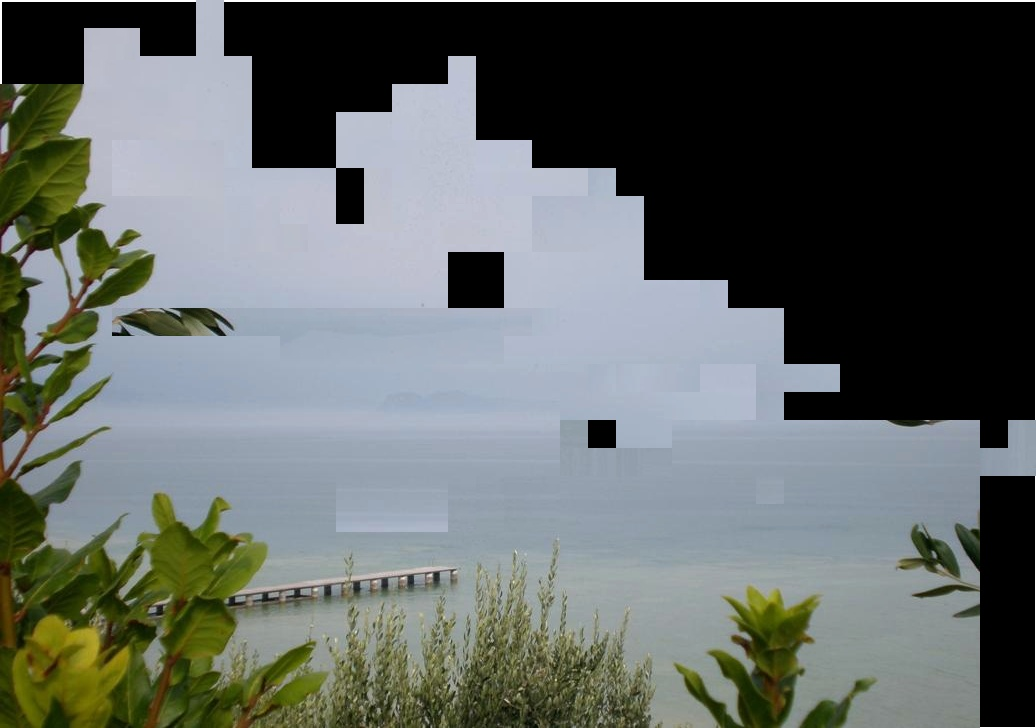
\includegraphics[scale=0.18]{./images/single_puzzle/reconstructed_805_3_01.jpg}} & \fbox{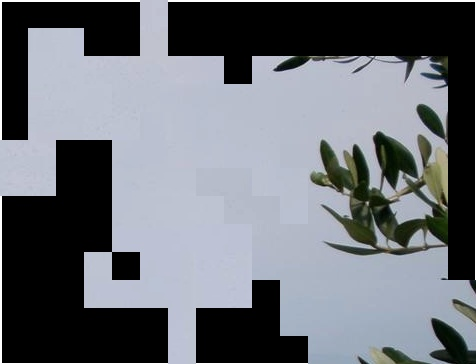
\includegraphics[scale=0.18]{./images/single_puzzle/reconstructed_805_3_02.jpg}} \\~\\
	MBS Output (a1) & MBS Output (a2) \\~\\
	
	\fbox{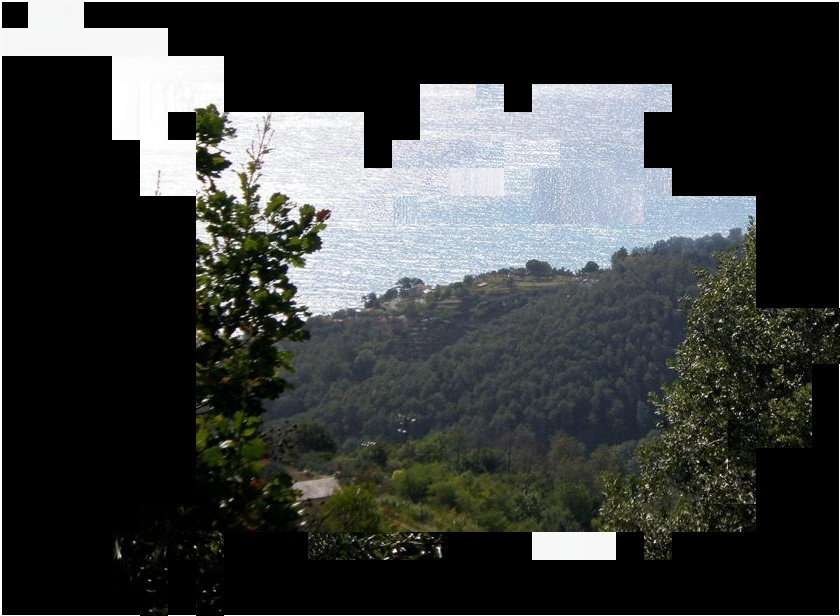
\includegraphics[scale=0.16]{./images/single_puzzle/reconstructed_805_12_01.jpg}} & \fbox{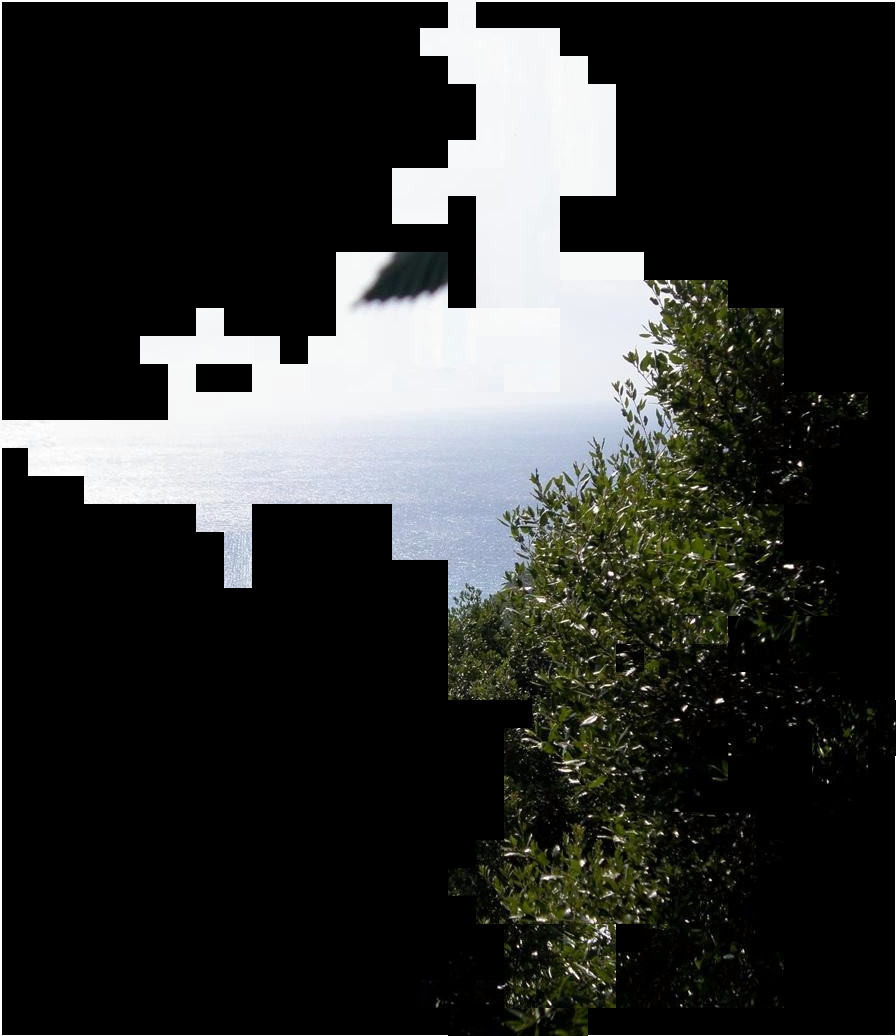
\includegraphics[scale=0.16]{./images/single_puzzle/reconstructed_805_12_02.jpg}} \\~\\
	MBS Output (b1) & MBS Output (b2) \\~\\
	
	\fbox{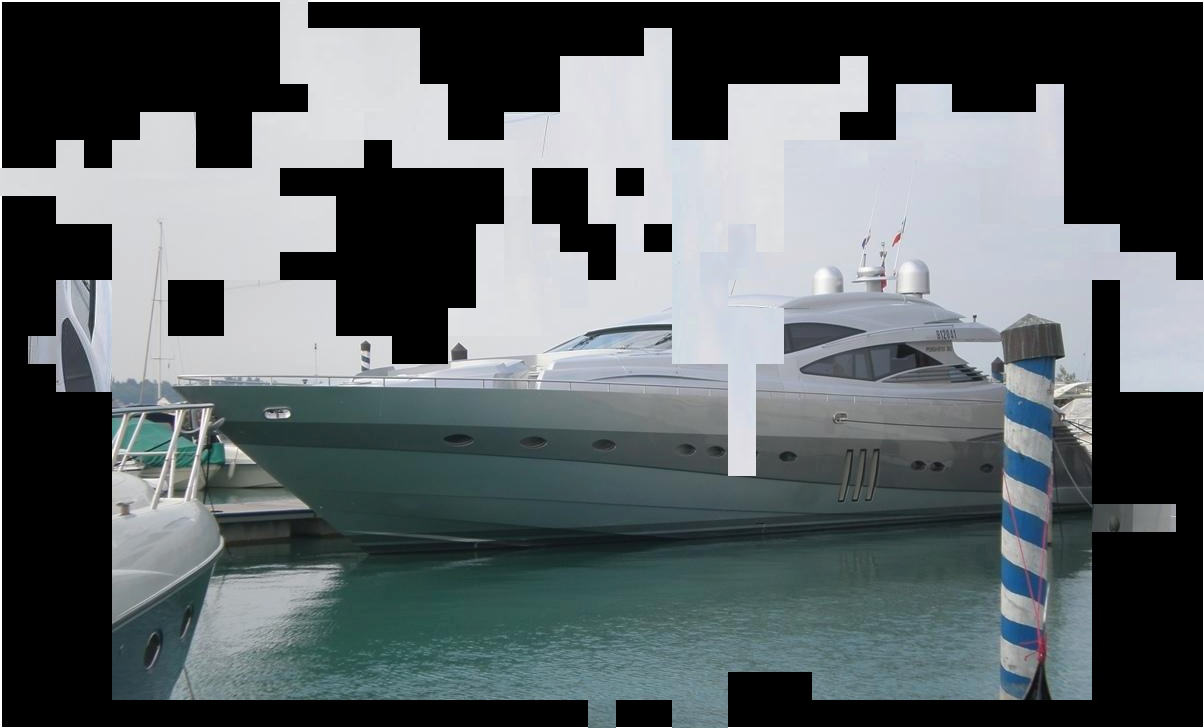
\includegraphics[scale=0.16]{./images/single_puzzle/reconstructed_805_16_01.jpg}} & \fbox{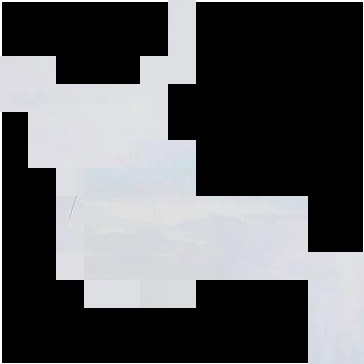
\includegraphics[scale=0.16]{./images/single_puzzle/reconstructed_805_16_02.jpg}} \\~\\
	MBS Output (c1) & MBS Output (c2) \\~\\
  \end{tabular}

\caption{Multi-Bag Solver Outputs for the Images not Correctly Identified as Single Inputs}
\label{fig:mixedBagSolverOuputsSingleImageIncorrectlyIdentified}
\end{figure}
